\documentclass[11pt]{article}
\usepackage[margin=1in]{geometry}

% Packages we need
\usepackage{amsmath}
\usepackage{amsfonts}
\usepackage{mathtools}
\usepackage{amsthm}
\usepackage{float}
\usepackage{graphicx}
\usepackage{listings}
\usepackage{color} %red, green, blue, yellow, cyan, magenta, black, white
\usepackage{animate}
 \usepackage{tikz} 
\usepackage{pgfplots}
\pgfplotsset{width=10cm,compat=1.9}
\usepgfplotslibrary{external}
\tikzexternalize

% Header packages
\usepackage{fancyhdr}
\fancyhf{}
\pagestyle{fancy}


% Formatting document
\setcounter{secnumdepth}{0}
\setlength{\parindent}{0in}
\setlength{\parskip}{0.5em}

% MATLAB code
\definecolor{mygreen}{RGB}{28,172,0} % color values Red, Green, Blue
\definecolor{mylilas}{RGB}{170,55,241}

% Commands
\DeclarePairedDelimiter\ceil{\lceil}{\rceil}
\DeclarePairedDelimiter\floor{\lfloor}{\rfloor}
\newcommand{\ws}{\text{ }}
\newcommand{\e}[1]{\times 10^{#1}}

% Header
\lhead{\textsc{CS 5220 -- Project 1}} % TODO: enter title here
\rhead{\textsc{Junteng Jia -- jj585\\Sania Nagpal -- sn579\\Bryce Evans -- bae43}} % Authors
\setlength{\headheight}{0.5in}
\cfoot{\thepage}

% Title
\title{CS 5220 -- Project 2} %TODO: enter title here
\author{
  \begin{tabular}{l c l}
    Junteng Jia  & -- & jj585 \\
    Sania Nagpal & -- & sn579 \\
    Bryce Evans  & -- & bae43 \\
  \end{tabular}\\
  \rule{\linewidth}{0.4pt}
}
\date{}

\lstset
{
    frame=tb,
    language=C++,
    aboveskip=3mm,
    belowskip=3mm,
    showstringspaces=false,
    columns=flexible,
    basicstyle={\small\ttfamily},
    numbers=none,
    numberstyle=\tiny\color{gray},
    keywordstyle=\color{blue},
    commentstyle=\color{dkgreen},
    stringstyle=\color{mauve},
    breaklines=true,
    breakatwhitespace=true,
    tabsize=4
}

\begin{document}
    \thispagestyle{empty}
    \maketitle
    \begin{center}
        \animategraphics[autoplay, loop, height=15cm]{10}{dam_break-}{0}{50}
    \end{center}
    \begin{center}
    This \texttt{Gif} shows the correctness of our code! Try open this report in acroread.
    \end{center}

    \clearpage
    
    \section{Our work}
        There are three major optimization base on the original code.
        \begin{enumerate}
            \item Profiling
            \item Parallelization
            \item Tuning
        \end{enumerate}
    
        \vspace{0.3cm}
                

        \section{Profiling}
        We did some hotspot analysis running the naive code, and this is what we find out:
        \begin{figure}[H]
            \centering
            \includegraphics[width=4.5in]{hotspot_previous.png}
            \caption{Previous hotspot analysis by amplxe-cl}
        \end{figure}
        
        The naive code is tested with one processor running the simulation on a 200 by 200 board.
        The board is surrounded by 4 layer of ghost cells, there is a synchronization every step.
        Which gives us a total of 208 by 208 simulation board. As you can see, the simulation time
        is around 1.4 second. \\
        
        We find that more than 58\% of time is spent on the function call $"$limited\_derivs$"$. 
        There are two reasons that cause this problem.
        \begin{itemize}
            \item First, because in previous code, "flux" is stored in an array of object, 
            when a block of memory is copied to cache, since an object of F or G has three field, 
            only $\frac{1}{3}$ of the memory is used in next step's calculation. 
            This leads to a lot of cache misses. 
            \item Second, because "flux" has to be accessed once every a few stride, 
            it is hard for compiler to fully utilize the power of vector register for calculation, 
            that is, copying and assmblying from cache to vector register is costly.
        \end{itemize}

        Before doing the profiling, our group checked the assmbly language of the hotspot, 
        this is what we find. According to the result, the bottleneck has already been vectorized
        by the compiler, however, the result shows that vectorization is not done correctly. 

        \clearpage
        
        \begin{figure}[H]
            \centering
            \includegraphics[width=4.5in]{assmbly_previous.png}
            \caption{Previous assmbly for hotspot}
        \end{figure}

    	Our current version of code is based on Prof. Bindel's C version of code. In our code,
        a lot of optimization has been added.
        
        \begin{itemize}
			\item \textbf{Data rearrangement:} In stead of using containers in C++, which create
            an array of objects, our current version of code uses an object of arrays to store the data
            of the simulation board. Each array contains a certain type of physical quantities.
            Therefore, when calculating the previous bottleneck $"$limited\_derivs$"$ function,
            data of two physically adjacent cells are continuous in memory.
            \item \textbf{Restricted pointer:} By using \texttt{restrict} to promise the compiler
            there is no other pointer pointing to the same memory with current pointer, the compiler
            is allowed to better optimize the code.
            \item \textbf{Step time:} We find out it is not necessary to calculate the maximum speed
            of cells to calculate the time step dt on the simulation board every time step. Since it
            doesn't change that much. Our previous version of code calculate the speed at the beginning
            of each frame and use that value for the whole frame.
            \item \textbf{Batch steps:} By adding multiple layer of ghost cells, and controlling the
            parameters (nx, ny, ng) at function $"$central2d\_step$"$, we are advancing multiple steps
            before synchronization. This is especially useful with we are running our code in parallel
            because barrier is very expensive. This gives us 25\% saving even running with single processor.
            \item \textbf{Optimizing loops:} We change the order of different loops to make sure in nested
            loops, processor are accessing continuous data in memory. On top of that, we create a variable
            in the outer loop to store the offset of the outer iterator, this reduces the function call of
            of $"$offset$"$ function and gives the compiler better opportunity to further vectorize the loop.
            Optimizing loops gives us around 10 \% saving.
            \clearpage
            \item \textbf{Inline functions:} We changes all the small-sized functions to inline, which saved
            the time for function going in and out the stack. We also tried change medium sized function to inline
            but it is refused by the compiler since it may cause oscillation between memory pages. 
		\end{itemize}
        
        After all those optimization, our code turns out to be 3-4 times faster than before. The time used for current 
        version of code is around 0.4 s for 50 frames of 200 by 200 simulation board. Note that there is synchronization
        overhead even when running with one thread. We did the hotspot analysis again.
        
        \begin{figure}[H]
            \centering
            \includegraphics[width=4.5in]{hotspot_current.png}
            \caption{Current hotspot analysis by amplxe-cl}
        \end{figure}
       
        Comparing with previous version of code, the hotspots of our current code is more balanced among different
        functions, which indicates there is no particular inappropriate performance error in our current version of
        code. We also checked the assmbly language. Our optimized code is completely vectorized on assmbly language level.
        
        \begin{figure}[H]
            \centering
            \includegraphics[width=4.0in]{assmbly_current.png}
            \caption{Current assmbly for hotspot}
        \end{figure}



        \section{Parallelization}
        We parallelized our code based on the domain decomposition idea. \texttt{SEP\_X} and \texttt{SEP\_Y} in the
        "ldrive.c" file indicate how many cut along one direction of the board. \\

        In our code, each thread has its own domain of simulation with \texttt{ng} layer of ghost cells.
        Well profiled $"$central2d\_t$"$ data structure is used as building blocks for parallelization.
        On top of that, we maintain an extra data structure $"$board2d\_t$"$ containing the water height and momentum
        of all the cells on the simulation board. Our $"$board2d\_t$"$ data structure is used for synchronization
        between different threads. \\
        
        There are three stages in each iteration of our parallel code:
        \begin{itemize}
            \item \texttt{Write\_in}: In this stage, each thread copy the periodic boundary to their own ghost cells.
            There is barrier at the end of this stage, so that no thread can modify the data of current simulation
            status on the global board until each thread has stored the data they need for simulation to their own
            local board. After this stage, each one of those subdomains is ready for simulation.
            \item \texttt{Central2d\_step}: In this stage, each thread do simulation on their own subdomain, and the
            water height and water speed of each cell is updated. This function is called twice per time to make sure
            the physical quantities finally local at the center of each cell. There is no synchronization in this stage,
            so the performance is decided by how well the serial code is profiled. the function $"$central2d\_step$"$
            is called several times in this stage before going into next stage of synchronization.
            \item \texttt{Write\_back}: In this stage, every thread copy their updated subdomain back to the global
            board data structure. There is a barrier after this stage to make sure before next iteration, the data 
            needed to fill in each subdomains' ghost cells is up-to-date.
        \end{itemize}

		To determine the performance of our parallelization, we ran the simulation on the cluster with different number
        of threads and different size of simulation board. We analyzed our result in terms of Strong scaling and weak
        scaling. On top of that, we tried to make the subdomain small so that the whole subdomain can fit into cache.
        Finally, bearing in mind the Xeon phi coprocessor has 60 unit of computational resources, we only plot the data
        in which the number of thread is below 60. \\
        
        Because the time used to simulate 1000 by 1000 board is much more than that of a 200 by 200 board, our data
        is separated into two plots to make sure the tendency is noticeable.
        
        \clearpage
        \vspace{0.5cm}
        
        \begin{center}
            \begin{tikzpicture}
                \begin{axis}[ xlabel=Number of treads, ylabel=time, xtick={0,1,4,9,16,25} ]
                \addplot plot coordinates 
                {
                    (1,    4.19771e-01)
                    (4,    1.45923e-01)
                    (9,    8.78133e-02)
                    (16,   9.95722e-02)
                    (25,   1.44698e-01)
                };
                \addplot plot coordinates 
                {
                    (1,    2.91779e-00)
                    (4,    9.74335e-01)
                    (9,    6.05319e-01)
                    (16,   6.55303e-01)
                    (25,   8.37134e-01)
                };
                \legend{$nx=ny=200$\\$nx=ny=400$\\}
                \end{axis}
            \end{tikzpicture}
        \end{center}

        \vspace{0.3cm}
        
        \begin{center}
            \begin{tikzpicture}
                \begin{axis}[ xlabel=number of treads, ylabel=time, xtick={0,1,4,9,16,25} ]
                \addplot plot coordinates 
                {
                    (1,    1.22312e+01)
                    (4,    2.90376e+00)
                    (9,    1.61187e+00)
                    (16,   1.66927e+00)
                    (25,   1.83527e+00)
                };
                \addplot plot coordinates 
                {
                    (1,    3.54752e+01)
                    (4,    7.93828e+00)
                    (9,    7.05672e+00)
                    (16,   8.20092e+00)
                    (25,   8.88018e+00)
                };
                \addplot plot coordinates 
                {
                    (1,    6.91330e+01)
                    (4,    2.73858e+01)
                    (9,    2.41228e+01)
                    (16,   2.81415e+01)
                    (25,   2.62972e+01)
                };
                \legend{$nx=ny=600$\\$nx=ny=800$\\$nx=ny=1000$\\}
                \end{axis}
            \end{tikzpicture}
        \end{center}
		
        \vspace{0.3cm}
        
    	The strong scaling analysis is shown by different points alone each line.
        \begin{itemize}
        	\item For different size of simulation board, the tendency is very similar.
            \item When the number of threads increases from 1 to 4, we get a factor of around 3. In the case of 200 by 200
            simulation board, we get a factor of 3.5.
            \item When the number of threads increases from 4 to 9, we only get a factor of 30\%. We think there are two
            reason for that:
            	\begin{itemize}
				\item First, we are using multiple layer of ghost cells, when the subdomain is small, the synchronization 
                and calculation overhead for ghost cells is comparably large. As the total amount of data goes up, the
                simulation subdomains can not all fit into cache thus increases the traffic between memory and cache, which
                is expensive comparing to cache access.
                \item Second, as the number of threads increase, the cost of barrier goes up, because all treads has to wait
                for the last one to finish.
                \end{itemize}
           	\item For the similar reason, we almost gain no performance when the number of threads increases further. When
            the number of threads goes beyond 8, the processor is begin hyperthreading, which should slow down because
            computational resource is shared between two threads. When the number of processor goes beyond 16, although openmp
            is a shared memory programming model, the memory is in reality distributed.
		\end{itemize}
        
        The plot below gives us the analysis of weak scaling.
        
        \begin{center}
            \begin{tikzpicture}
                \begin{axis}[ xlabel=number of treads, ylabel=time, xtick={0,1,4,9,16,25} ]
                \addplot plot coordinates 
                {
                    (1,    4.19771e-01)
                    (4,    9.74335e-01)
                    (9,    1.61187e+00)
                    (16,   8.20092e+00)
                    (25,   2.62972e+01)
                };
                \legend{200 by 200 per thread\\}
                \end{axis}
            \end{tikzpicture}
        \end{center}
		
        \begin{itemize}
        	\item When the number of threads goes from 1 to 4 to 9 the weak scaling diagram is not perfect but acceptable. 
            This is because:
            	\begin{itemize}
					\item The simulation board can no longer fit into L2 cache, and memory access is costly.
				\end{itemize}
        	\item When the number of threads goes from 9 to 16, the scaling is much worse, it is because:
            	\begin{itemize}
					\item The simulation boards can not even fit into the L3 cache.
                    \item Hyperthreading does not equal real computation power.
				\end{itemize}
            \item When the number of threads goes from 16 to 25, the scaling is very bad, it is because:
            	\begin{itemize}
                    \item Accessing distributed memory is very expensive.
				\end{itemize}
		\end{itemize}
  
  		The reason that weak scaling is not so good in our program is that we didn't consider the communication between
        distributed memory. This justified the remark by Prof. Bindel "There is a best way to do OPENMP, that's MPI."

	\section{Tuning}
	We tuned our code against the batch size. Large number of batch reduces the synchronization, however, it increases
    the amount of calculation and memory usage. It turns out the best batch steps strategy is to synchronize once after
    running $"$central2d\_step$"$ 10 time, which requires 16 layers of ghost cells.
    
    \section{Summary}
    Our code gives a good serial performance, and the parallel performance is also good for small number of threads ($\leq$9).
    When the number of threads is bigger than 9, for the reason we have discussed, the performance is not as good.
    
    Through this project:
    \begin{itemize}
        \item We analyzed the hotspot of our code through profiling. We learned to use data rearrangement, inline, restrict
        pointer to help compiler optimize our code. We learned to use more layer of ghost cells and bigger batch size to
        reduce synchronization.
        \item We learned how to use strong scaling and weak scaling paradigm to analysis the performance of parallel code.
        \item We noticed the importance of using MPI for distributed memory communication.
    \end{itemize}

	If we have more time on this project:
    \begin{itemize}
    	\item We will try to use MPI for inter node communication, OPENMP for intra node communication to further optimize our
        code.
    \end{itemize}
\end{document}

